%%%%%%%%%%%%%%%%%%%%%%%%%%%%%%%%%%%%%%%%%
% Friedrich M. Grabner - 01220997
% HPC Coursework
%%%%%%%%%%%%%%%%%%%%%%%%%%%%%%%%%%%%%%%%%

%----------------------------------------------------------------------------------------
%	PACKAGES AND DOCUMENT CONFIGURATIONS
%----------------------------------------------------------------------------------------
\documentclass[10pt, a4paper]{article}
\usepackage{amsmath, amsthm, amssymb}
\usepackage{graphicx} % Required for the inclusion of images
\usepackage{natbib} % Required to change bibliography style to APA
\usepackage{nomencl}
\usepackage{setspace}
\usepackage{geometry} 
\usepackage{hyperref}
\usepackage{subcaption}
\usepackage{xcolor}
\usepackage{lmodern}
\usepackage{listings}
\lstset{language=[90]Fortran,
  basicstyle=\ttfamily,
  keywordstyle=\color{red},
  commentstyle=\color{green},
  morecomment=[l]{!\ }% Comment only with space after !
}

\geometry{a4paper,total={170mm,257mm},left=20mm,top=20mm}



\setlength\parindent{5pt} % Removes all indentation from paragraphs
\graphicspath{{./images/}}
\DeclareGraphicsExtensions{.pdf,.PDF,.jpg,.JPG,.bmp,.png,.eps,.EPS}

%\usepackage{times} % Uncomment to use the Times New Roman font

\input{/home/fmg215/Documents/latex/symbols.tex}
%----------------------------------------------------------------------------------------
%	DOCUMENT INFORMATION
%----------------------------------------------------------------------------------------
\newcommand*{\plogo}{\fbox{$\mathcal{PL}$}}

\newcommand*{\titleGM}{\begingroup % Create the command for including the title page in the document
\hbox{ % Horizontal box
\hspace*{0.2\textwidth} % Whitespace to the left of the title page
\rule{1pt}{\textheight} % Vertical line
\hspace*{0.05\textwidth} % Whitespace between the vertical line and title page text
\parbox[b]{0.75\textwidth}{ % Paragraph box which restricts text to less than the width of the page

{\noindent\huge\bfseries High Performance Computing \\[0.5\baselineskip] AE3-422}\\[2\baselineskip] % Title
{\Large \textsc{F. M. Grabner - 01220997}}\\[4\baselineskip] % Tagline or further description
{\large } % Author name

\vspace{0.5\textheight} % Whitespace between the title block and the publisher
{\noindent Imperial College London - Department of Aeronautics}\\[\baselineskip] % Publisher and logo
}}
\endgroup}
%----------------------------------------------------------------------------------------
%	TITLE PAGE
%----------------------------------------------------------------------------------------
\begin{document}
\titleGM
%----------------------------------------------------------------------------------------
%	QUESTION 1
%----------------------------------------------------------------------------------------
\section*{Question 1}
Figure \ref{fig:task1} shows the analytical solution against computed solution using the static equations. The computed solution shows strong correlation to that of the analytical.

\begin{figure}[!htb]
  \centering
	  \includegraphics[width=.5\linewidth, clip=true, trim=0cm 0cm 0cm 0cm]{task1}
  \caption{Static against analytical solutions.}
  \label{fig:task1}
\end{figure}%

Matrices have been set up in banded format to minimise the memory footprint. Then the system is solved utilising Lapack\cite{Lapack1999} function DGBSV. However to utilise the Fortran routines in BLAS\cite{Blas1979}, column-major storage format has been utilised which goes against natural C++ format.

%----------------------------------------------------------------------------------------
%	QUESTION 2
%----------------------------------------------------------------------------------------
\section*{Question 2}

For task 2 the solution was found using an explicit central-difference scheme. As in task 1 banded storage was utilised and BLAS level 3 routine dgbmv in order to find the solution.

\begin{figure}[!htb]
\centering
\begin{subfigure}{.5\textwidth}
  \centering
  \includegraphics[width=1\linewidth]{task2_amplitude}
  \caption{Amplitude of oscillations.}
  \label{fig:amplitude2}
\end{subfigure}%
\begin{subfigure}{.5\textwidth}
  \centering
  \includegraphics[width=1\linewidth]{task2_deflection}
  \caption{Oscilation with different loading factors.}
  \label{fig:deflection2}
\end{subfigure}
\caption{Grid Independence Test.}
\label{fig:task2}
\end{figure}

Figure \ref{fig:deflection2} shows the deflection at the midpoint against time, for a number of different loading times. To the left of which is figure \ref{fig:amplitude2} which shows the amplitude of oscillations as the loading time is increased from time $0 - 1 (s)$ in steps of size $\Delta t = 0.001 s$. As load time increases the amplitude of oscillations decrease. However 
%----------------------------------------------------------------------------------------
%	QUESTION 3
%----------------------------------------------------------------------------------------
\section*{Question 3}

Task 3 required the system to be solved using the Newmark implicit integration scheme. Again all matrices were created in banded format and solved using BLAS level 3 routines.

\begin{figure}[!htb]
\centering
\begin{subfigure}{.5\textwidth}
  \centering
  \includegraphics[width=1\linewidth]{task3_amplitude}
  \caption{Amplitude of oscillations.}
  \label{fig:amplitude3}
\end{subfigure}%
\begin{subfigure}{.5\textwidth}
  \centering
  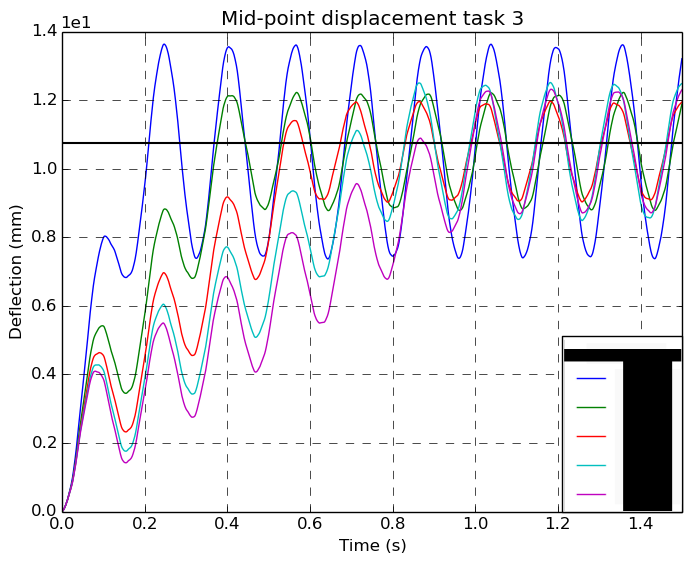
\includegraphics[width=1\linewidth]{task3_deflection}
  \caption{Oscilation with different loading factors.}
  \label{fig:deflection3}
\end{subfigure}
\caption{Grid Independence Test.}
\label{fig:task3}
\end{figure}

Using the implicit scheme the beam exhibits an almost identical response to that of the explicit integration scheme, which is to be expected. Again some sort of frequency response is seen in that certain frequencies have significantly lower amplitude than others however the general trend is to an oscillation at order of magnitude $\approx 1mm$.

However with the Newmark method a solution is found using far fewer time steps due to the implicit nature of the scheme.

%----------------------------------------------------------------------------------------
%	QUESTION 4
%----------------------------------------------------------------------------------------
\section*{Question 4}

In task 4 the beam was solved across multiple processors. To do so MPI has been implemented into the code and the domain split between processors. In order to keep the problem size as small as possible but still keep an even distribution across nodes, the domain has been split with an overlap region at the centre-point. The system is solved using the dgemv on a single core and exchanging contributions at the end of each time step. However from the upper rank the overlap contributions must be ignored to keep the system correct.

\begin{figure}[!htb]
  \centering
	  \includegraphics[width=.5\linewidth, clip=true, trim=0cm 0cm 0cm 0cm]{task4_timing}
  \caption{Time to solution as problem size increases with 1 and 2 processors.}
  \label{fig:timing4}
\end{figure}%

Above figure \ref{fig:timing4} shows the time to solution for different problem sizes. Clear to see that except for small problems less than 200 elements the MPI routines are significantly quicker.

%----------------------------------------------------------------------------------------
%	QUESTION 5
%----------------------------------------------------------------------------------------
\section*{Question 5}

\begin{figure}[!htb]
  \centering
	  \includegraphics[width=.5\linewidth, clip=true, trim=0cm 0cm 0cm 0cm]{task5_timing}
  \caption{Time to solution as problem size increases with 1, 2 and 4 processors.}
  \label{fig:timing5}
\end{figure}%

%---------------------------------------------------------------------------------------
%	BIBLIOGRAPHY
% ---------------------------------------------------------------------------------------
\bibliographystyle{unsrt}	% in order of appearance
%\bibliographystyle{acm}	% (uses file "plain.bst")
%\bibliographystyle{abbrv}	% (uses file "plain.bst")
%\bibliographystyle{siam}	% (uses file "plain.bst")
%\bibliographystyle{apalike}
\bibliography{/home/fmg215/Documents/latex/myrefs}		% expects file "myrefs.bib"}
%----------------------------------------------------------------------------------------
% END DOCUMENT
%----------------------------------------------------------------------------------------
\end{document}